\section{User and System Time Histograms on the Second Run~\label{sec:u_s_time_hist}} 
This section exhibits user and system time histograms on the second run of 
INC with its task length increasing from 1 second to 4096 seconds, via SEDONA. 
The detailed description of the base data is from Table~\ref{tab:exp_notes2}.

\subsection{User Time}

\begin{figure}[hp!]
	\centering
	\subfigure[User time frequency on INC1]{
		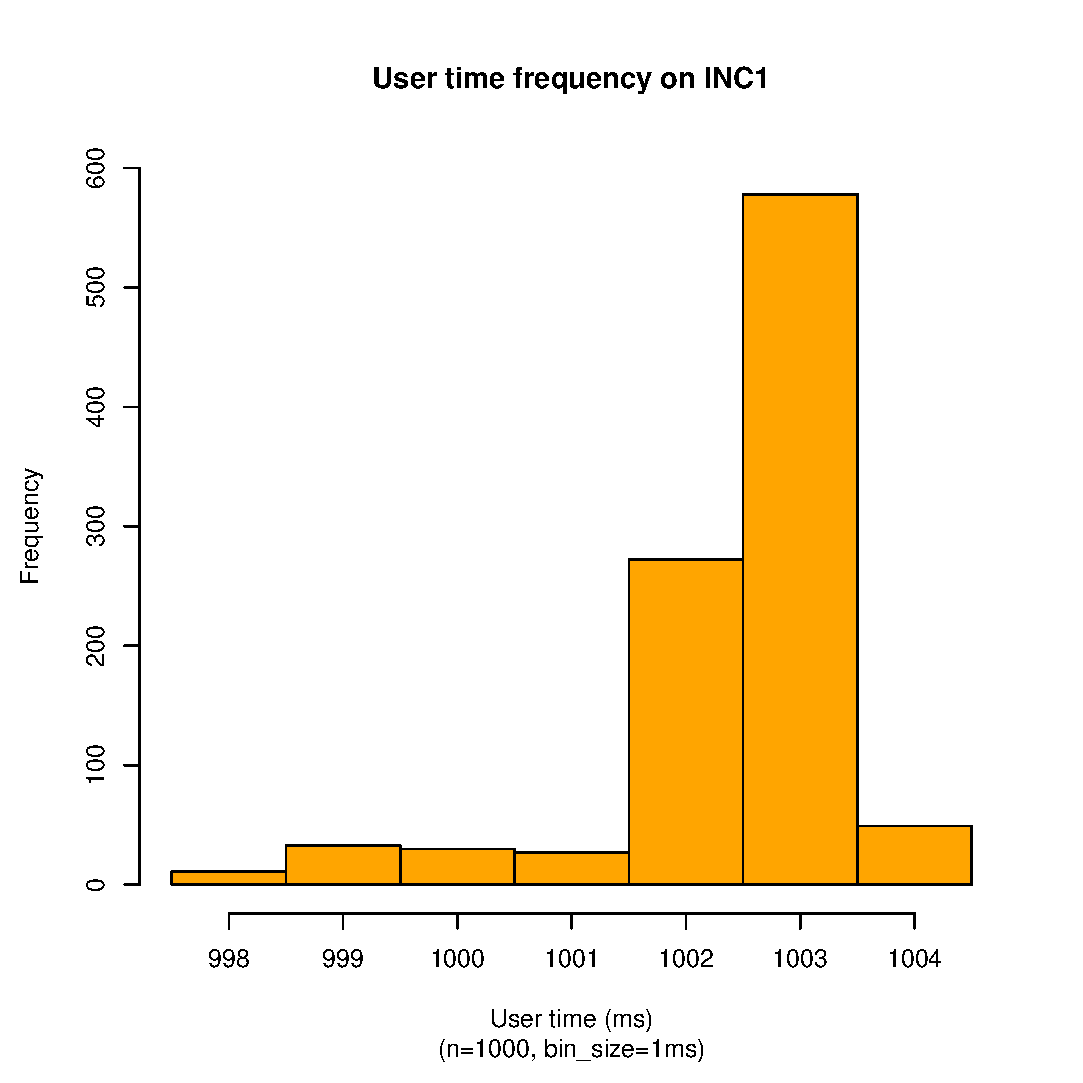
\includegraphics[scale=0.43]{u_s_time/1_sec_ut_hist.eps}
		\label{fig:inc1_ut_hist}
	}
	\subfigure[User time frequency on INC2]{
		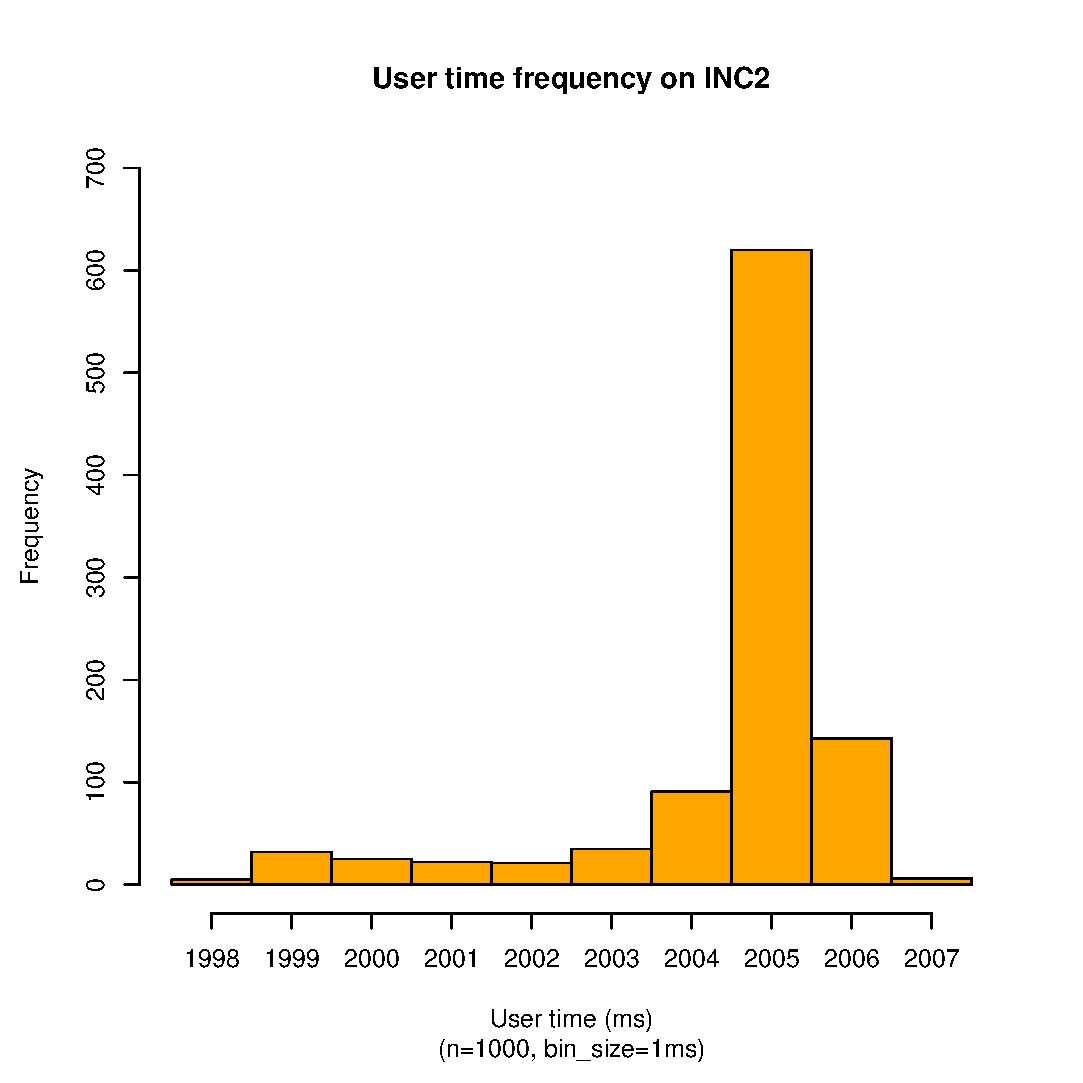
\includegraphics[scale=0.43]{u_s_time/2_sec_ut_hist.eps}
		\label{fig:inc2_ut_hist}
	}
	\subfigure[User time frequency on INC4]{
		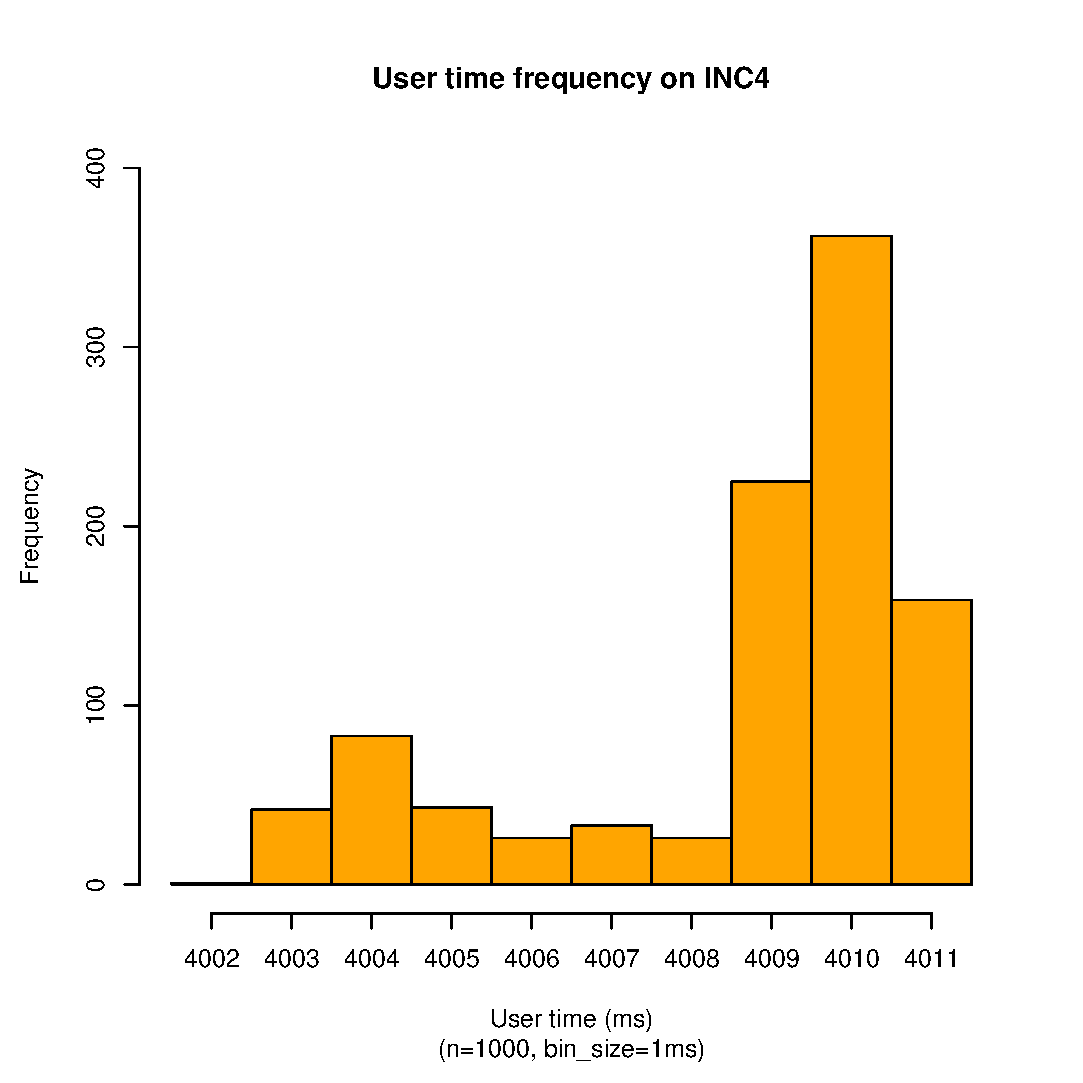
\includegraphics[scale=0.43]{u_s_time/4_sec_ut_hist.eps}
		\label{fig:inc4_ut_hist}
	}
	\subfigure[User time frequency on INC8]{
		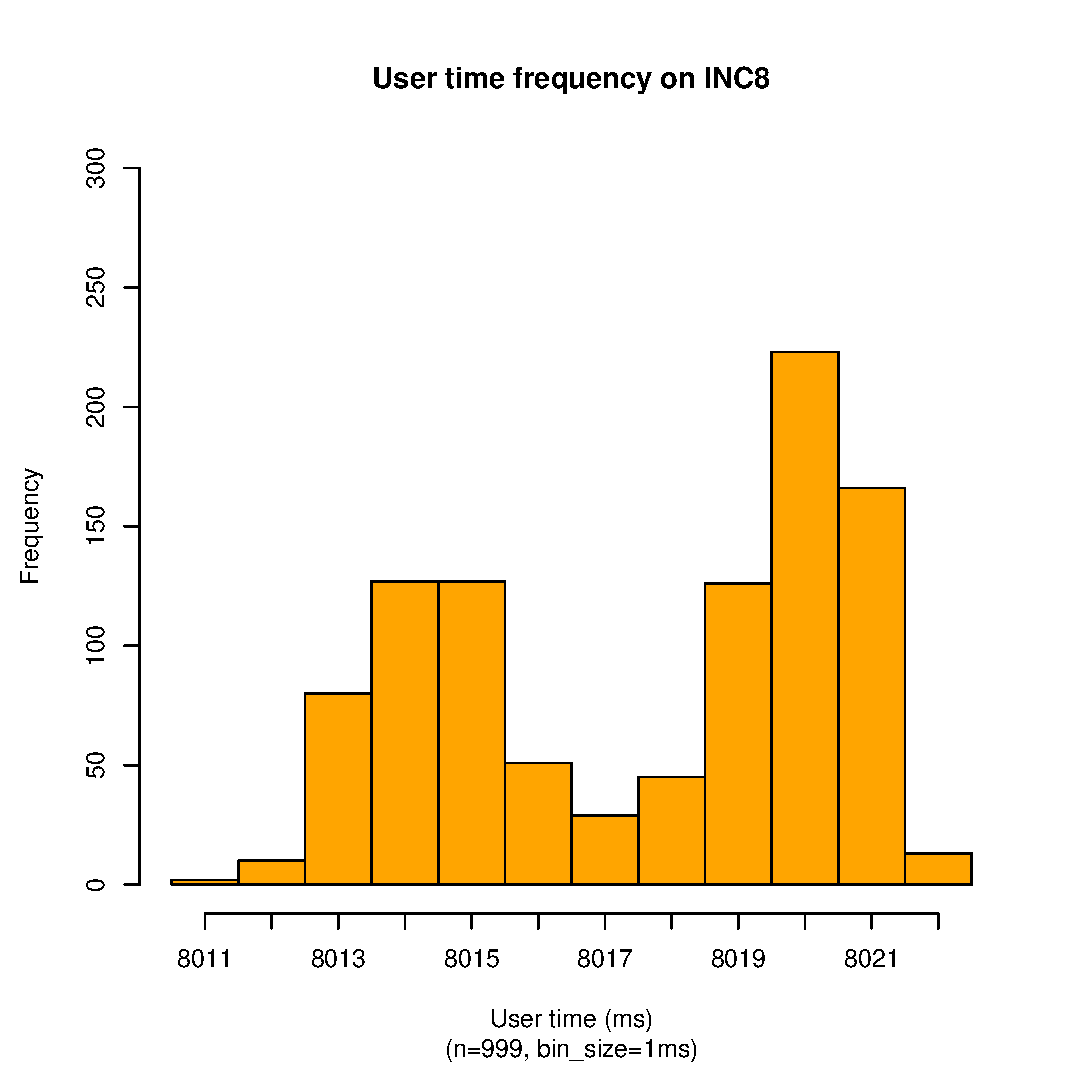
\includegraphics[scale=0.43]{u_s_time/8_sec_ut_hist.eps}
		\label{fig:inc8_ut_hist}
	}
	\caption{User Time Histograms of INC1 ... INC8~\label{fig:ut_hist1}}
\end{figure}

\begin{figure}[hp!]
	\centering
	\subfigure[User time frequency on INC16]{
		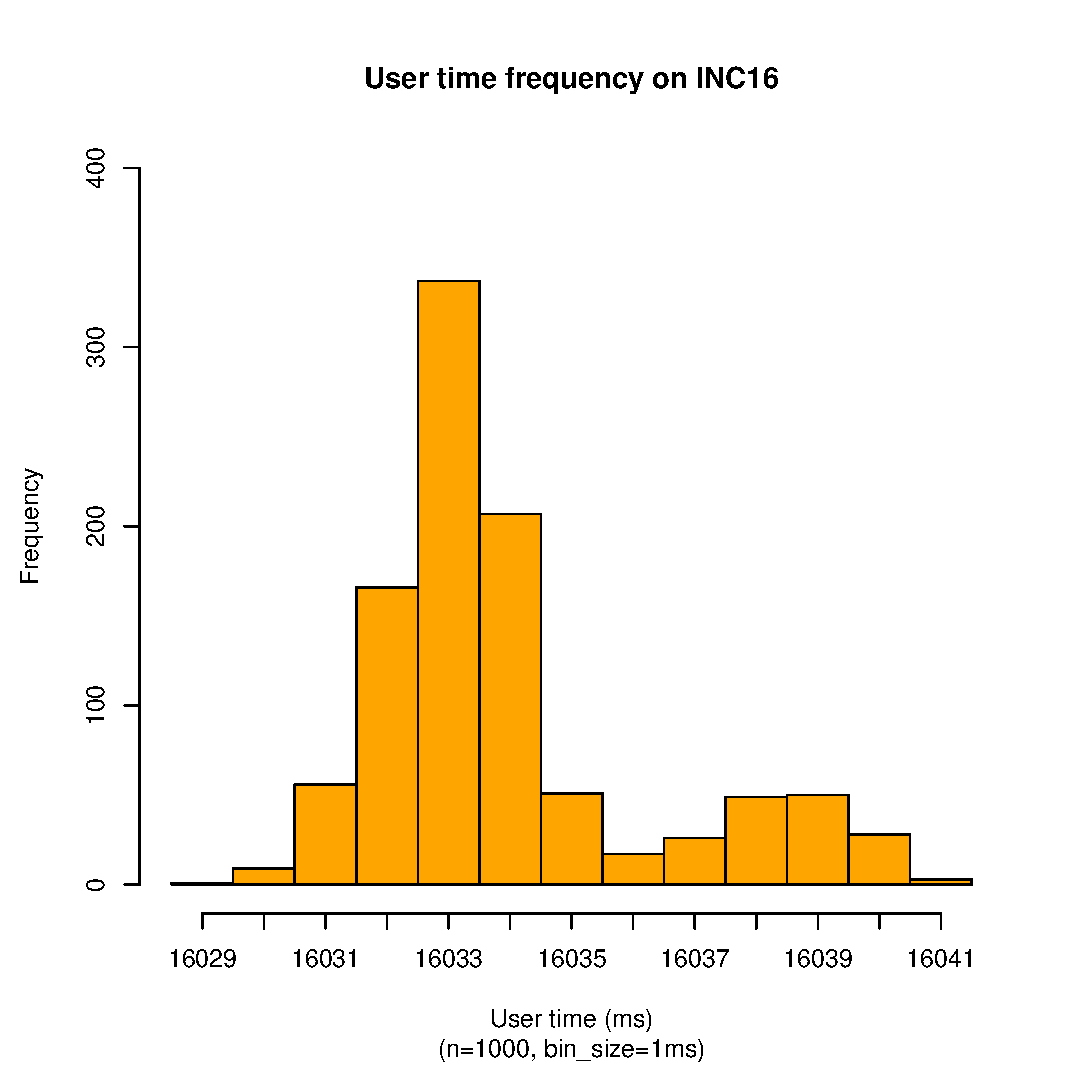
\includegraphics[scale=0.43]{u_s_time/16_sec_ut_hist.eps}
		\label{fig:inc16_ut_hist}
	}
	\subfigure[User time frequency on INC32]{
		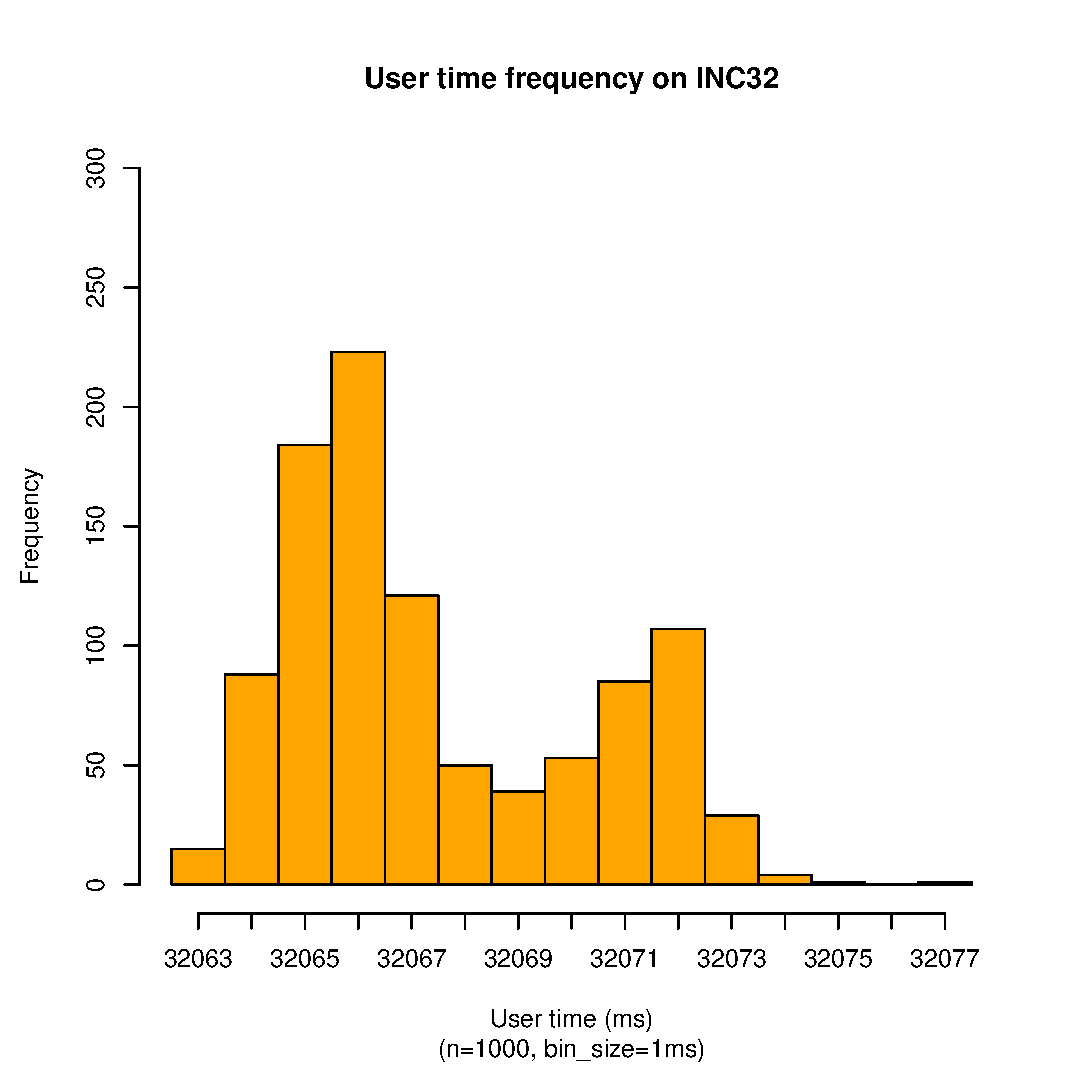
\includegraphics[scale=0.43]{u_s_time/32_sec_ut_hist.eps}
		\label{fig:inc32_ut_hist}
	}
	\subfigure[User time frequency on INC64]{
		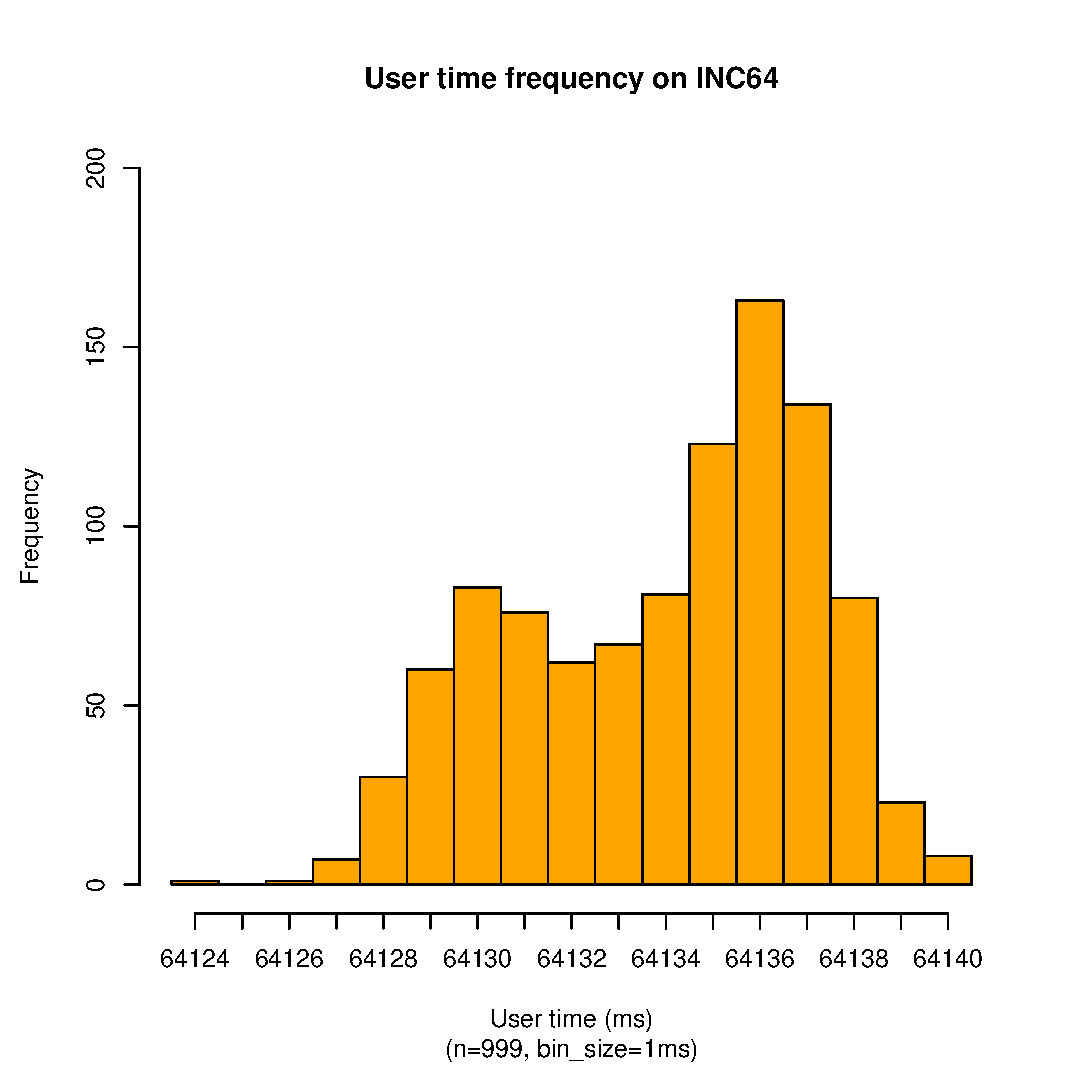
\includegraphics[scale=0.43]{u_s_time/64_sec_ut_hist.eps}
		\label{fig:inc64_ut_hist}
	}
	\caption{User Time Histograms of INC16 ... INC64~\label{fig:ut_hist2}}
\end{figure}

\begin{figure}[hp!]
	\centering
	\subfigure[User time frequency on INC128]{
		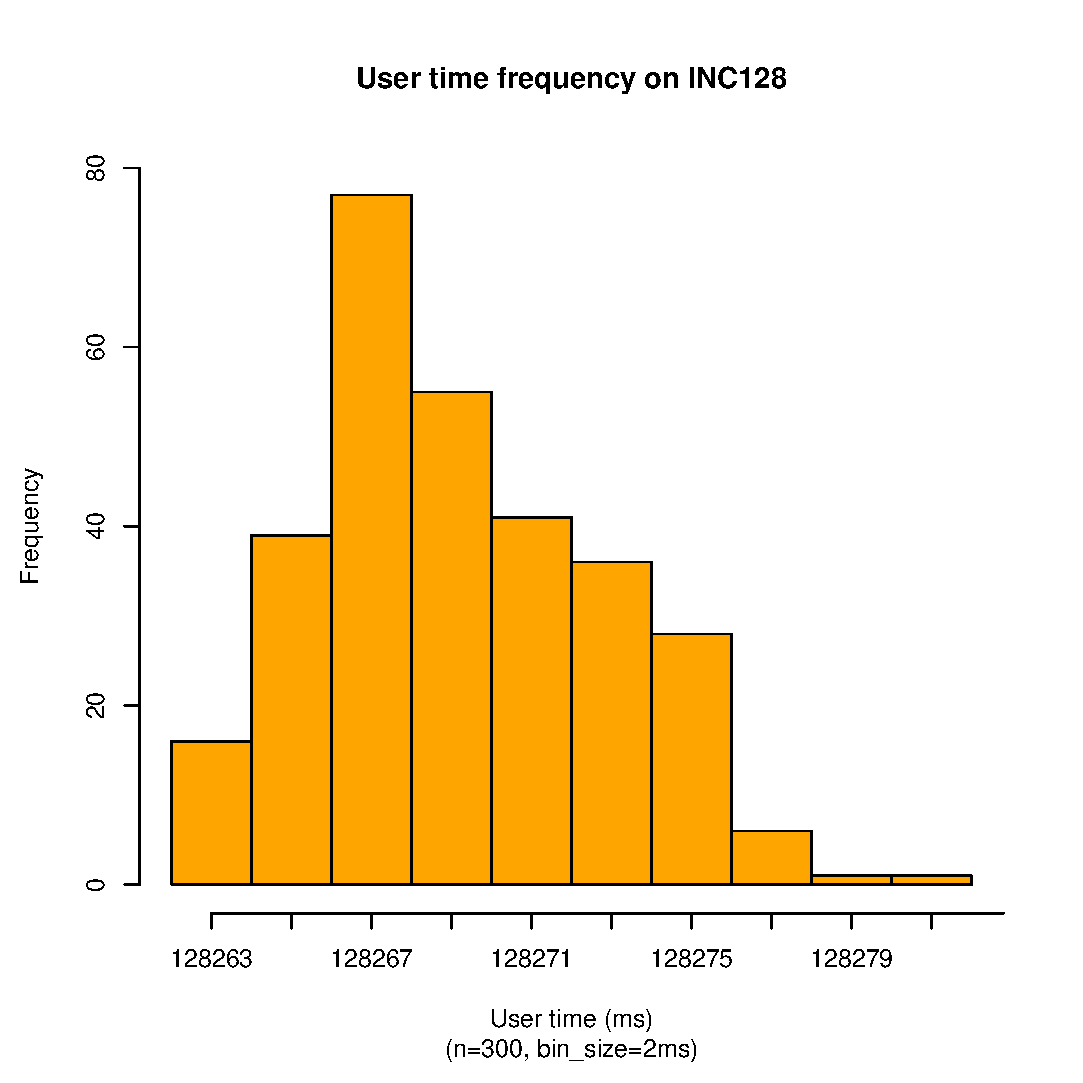
\includegraphics[scale=0.43]{u_s_time/128_sec_ut_hist.eps}
		\label{fig:inc128_ut_hist}
	}
	\subfigure[User time frequency on INC256]{
		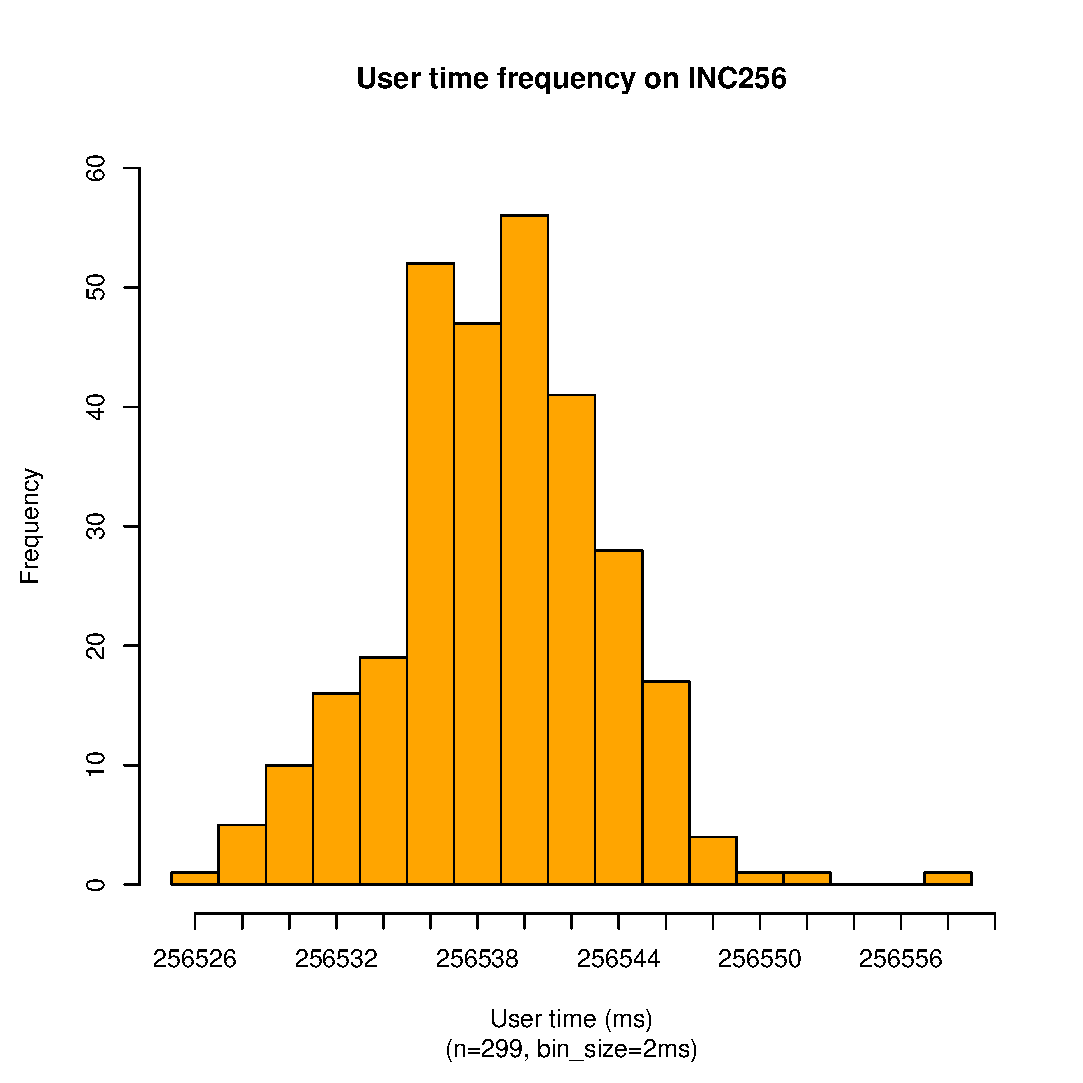
\includegraphics[scale=0.43]{u_s_time/256_sec_ut_hist.eps}
		\label{fig:inc256_ut_hist}
	}
	\subfigure[User time frequency on INC512]{
		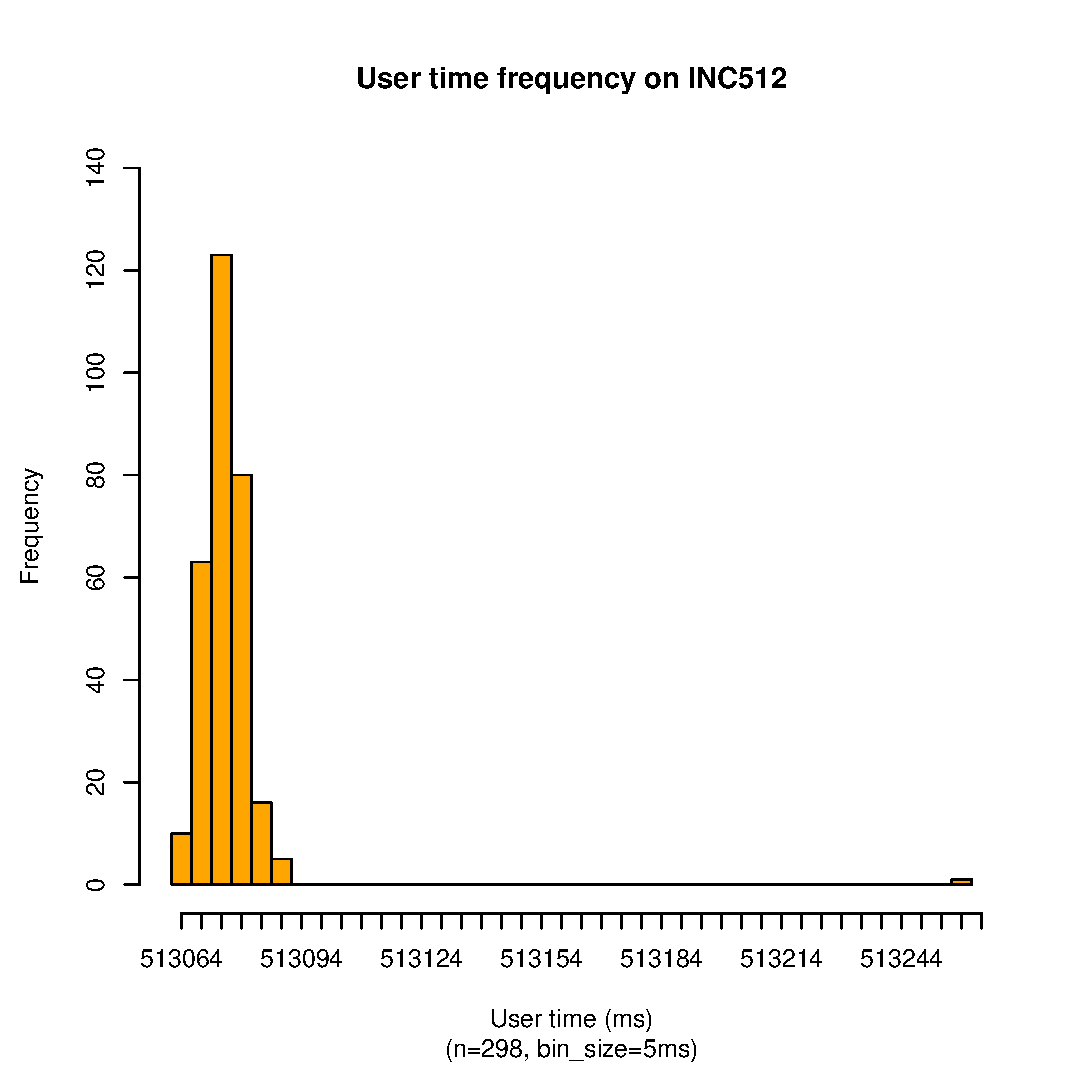
\includegraphics[scale=0.43]{u_s_time/512_sec_ut_hist.eps}
		\label{fig:inc512_ut_hist}
	}
	\subfigure[User time frequency on INC1024]{
		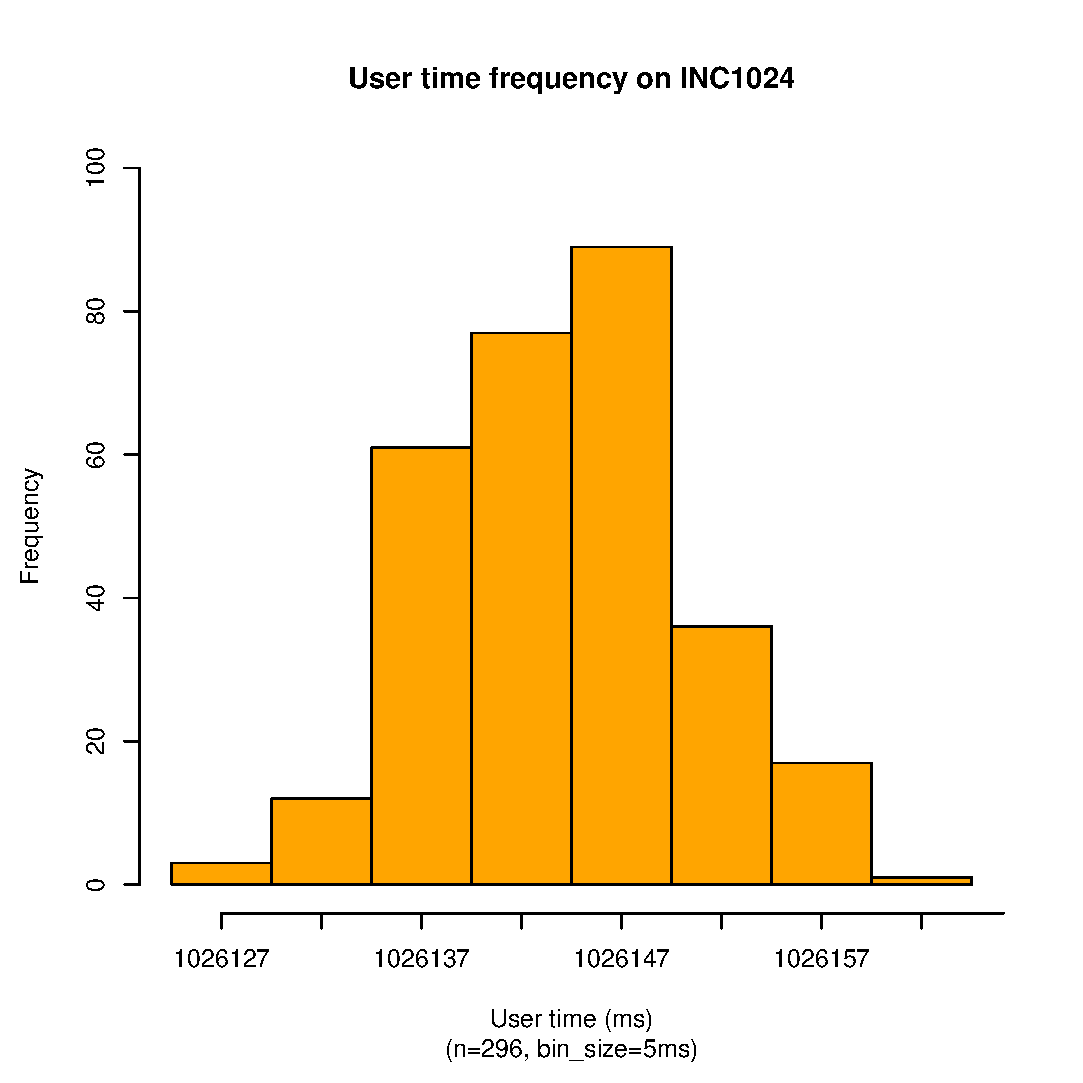
\includegraphics[scale=0.43]{u_s_time/1024_sec_ut_hist.eps}
		\label{fig:inc1024_ut_hist}
	}
	\caption{User Time Histograms of INC128 ... INC1024~\label{fig:ut_hist3}}
\end{figure}

\begin{figure}[hp!]
	\centering
	\subfigure[User time frequency on INC2048]{
		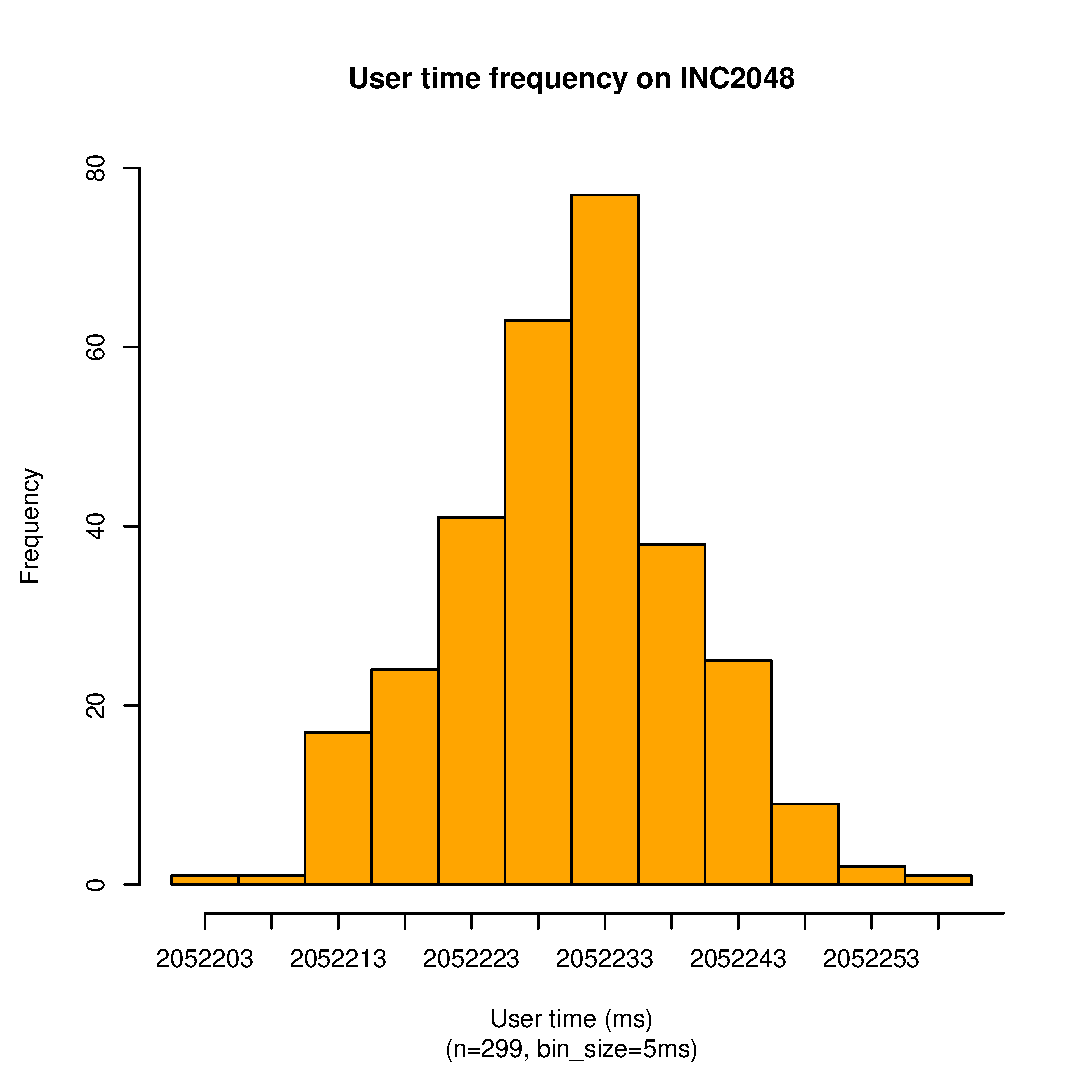
\includegraphics[scale=0.43]{u_s_time/2048_sec_ut_hist.eps}
		\label{fig:inc2048_ut_hist}
	}
	\subfigure[User time frequency on INC4096]{
		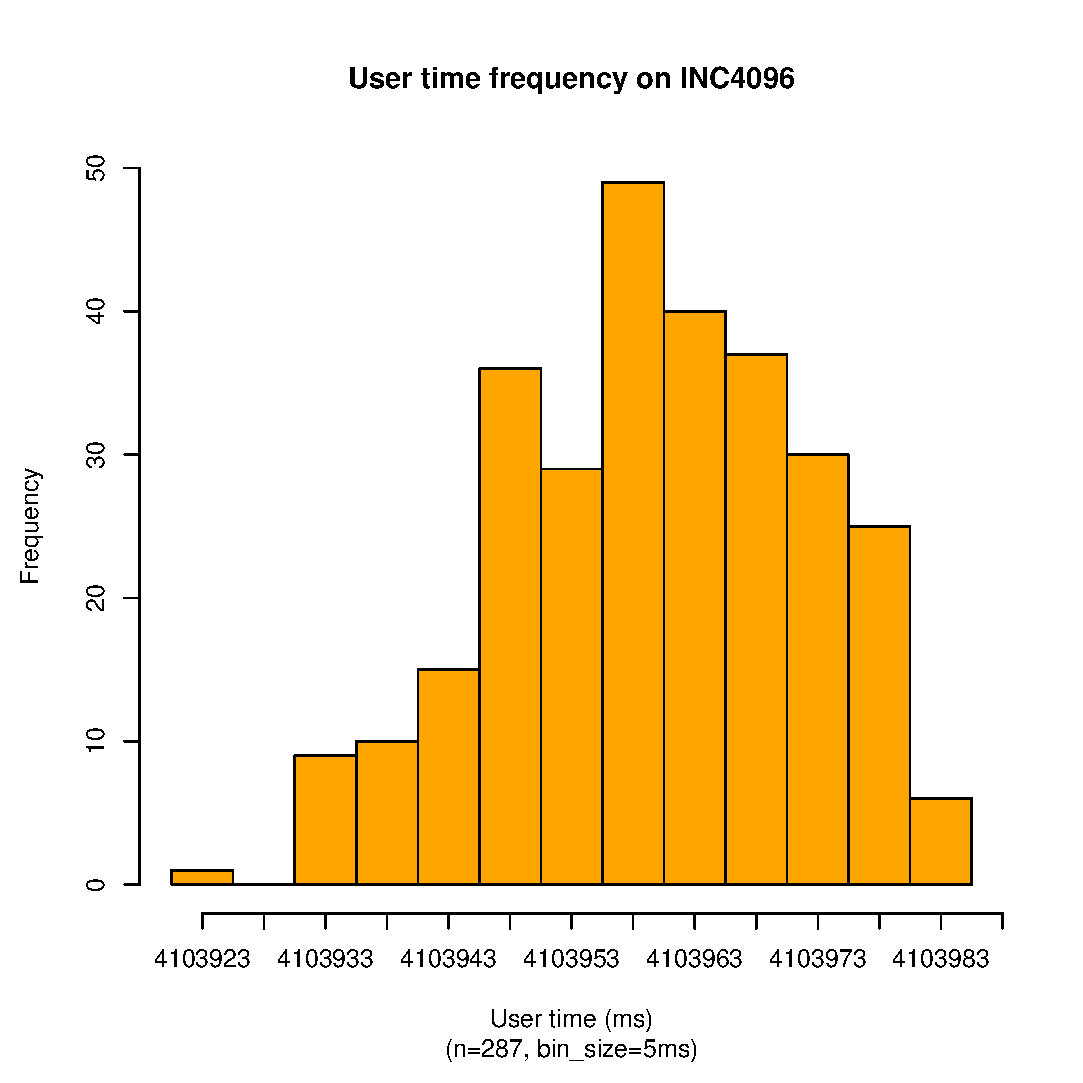
\includegraphics[scale=0.43]{u_s_time/4096_sec_ut_hist.eps}
		\label{fig:inc4096_ut_hist}
	}
	\caption{User Time Histograms of INC2048 and INC4096~\label{fig:ut_hist4}}
\end{figure}

\vspace\fill
\clearpage

\subsection{System Time}

\begin{figure}[hp!]
	\centering
	\subfigure[System time frequency on INC1]{
		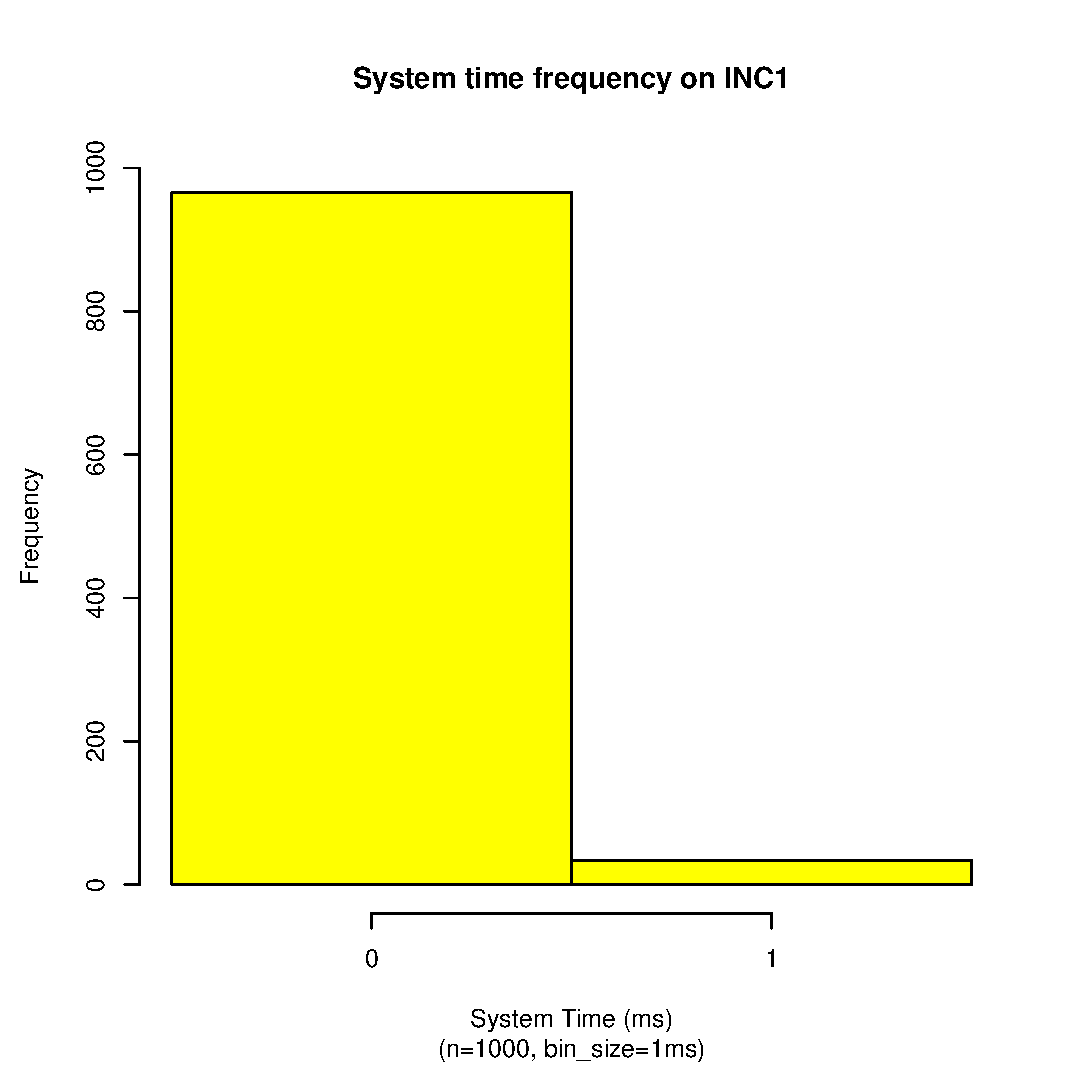
\includegraphics[scale=0.43]{u_s_time/1_sec_st_hist.eps}
		\label{fig:inc1_hist_v5}
	}
	\subfigure[System time frequency on INC2]{
		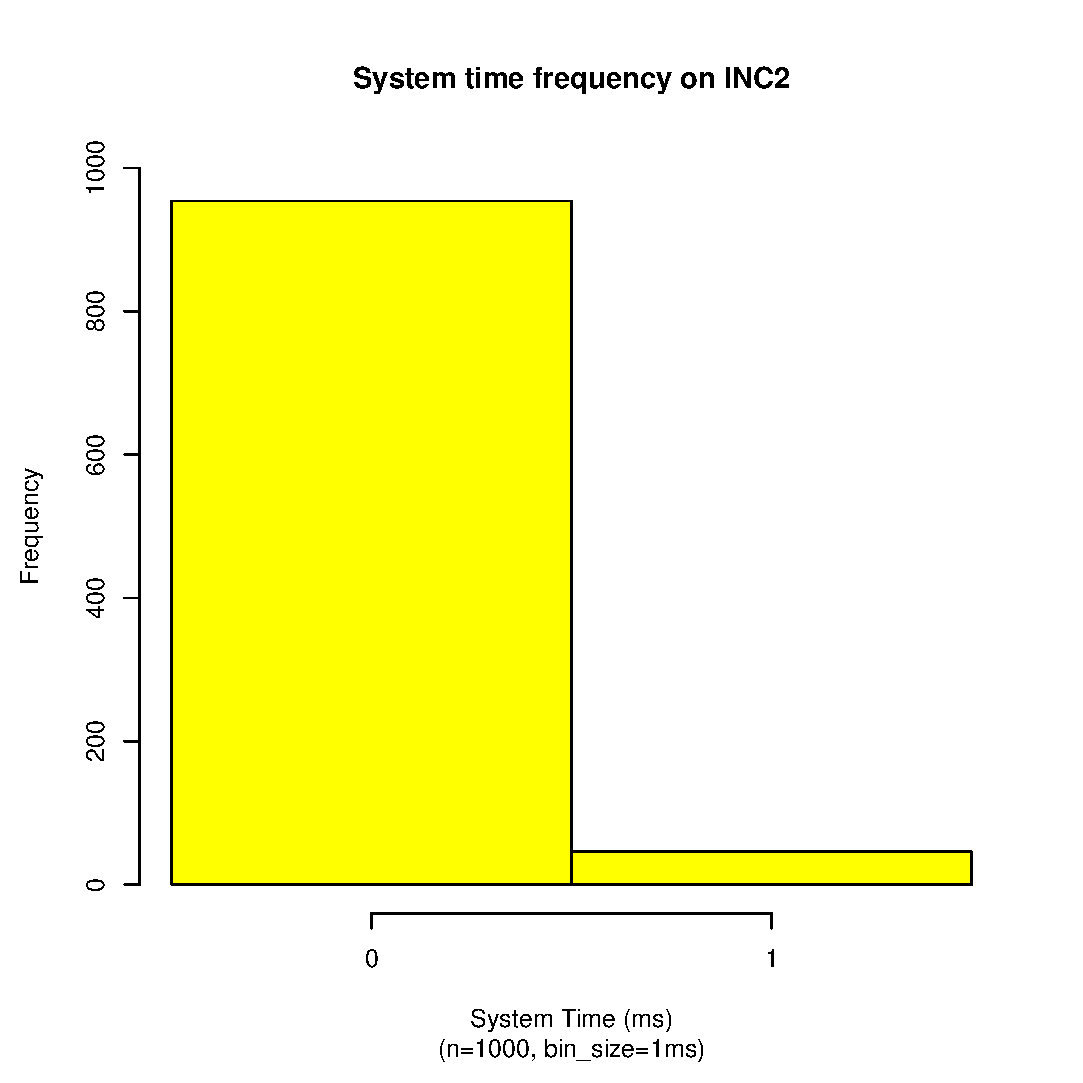
\includegraphics[scale=0.43]{u_s_time/2_sec_st_hist.eps}
		\label{fig:inc2_hist_st}
	}
	\subfigure[System time frequency on INC4]{
		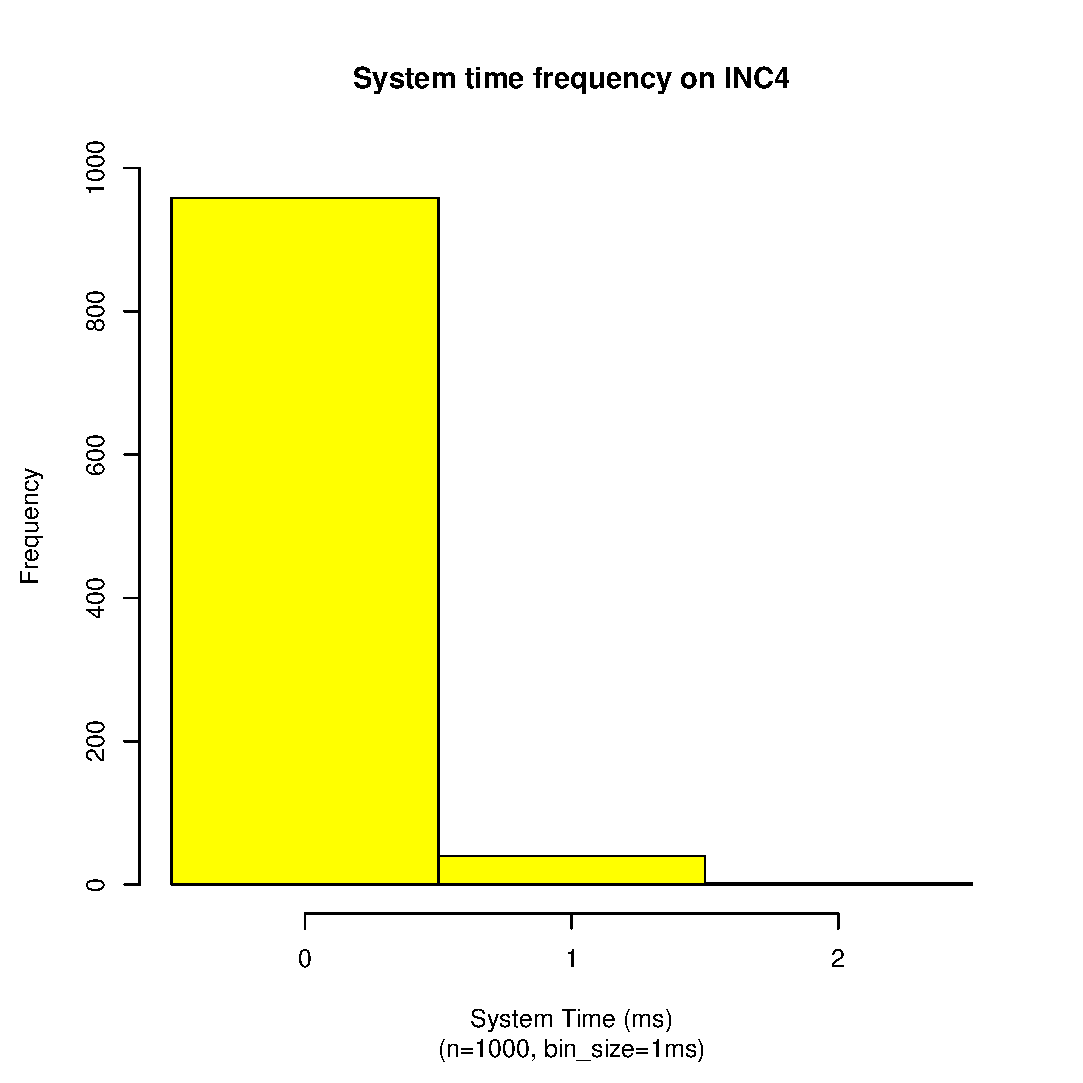
\includegraphics[scale=0.43]{u_s_time/4_sec_st_hist.eps}
		\label{fig:inc4_hist_st}
	}
	\subfigure[System time frequency on INC8]{
		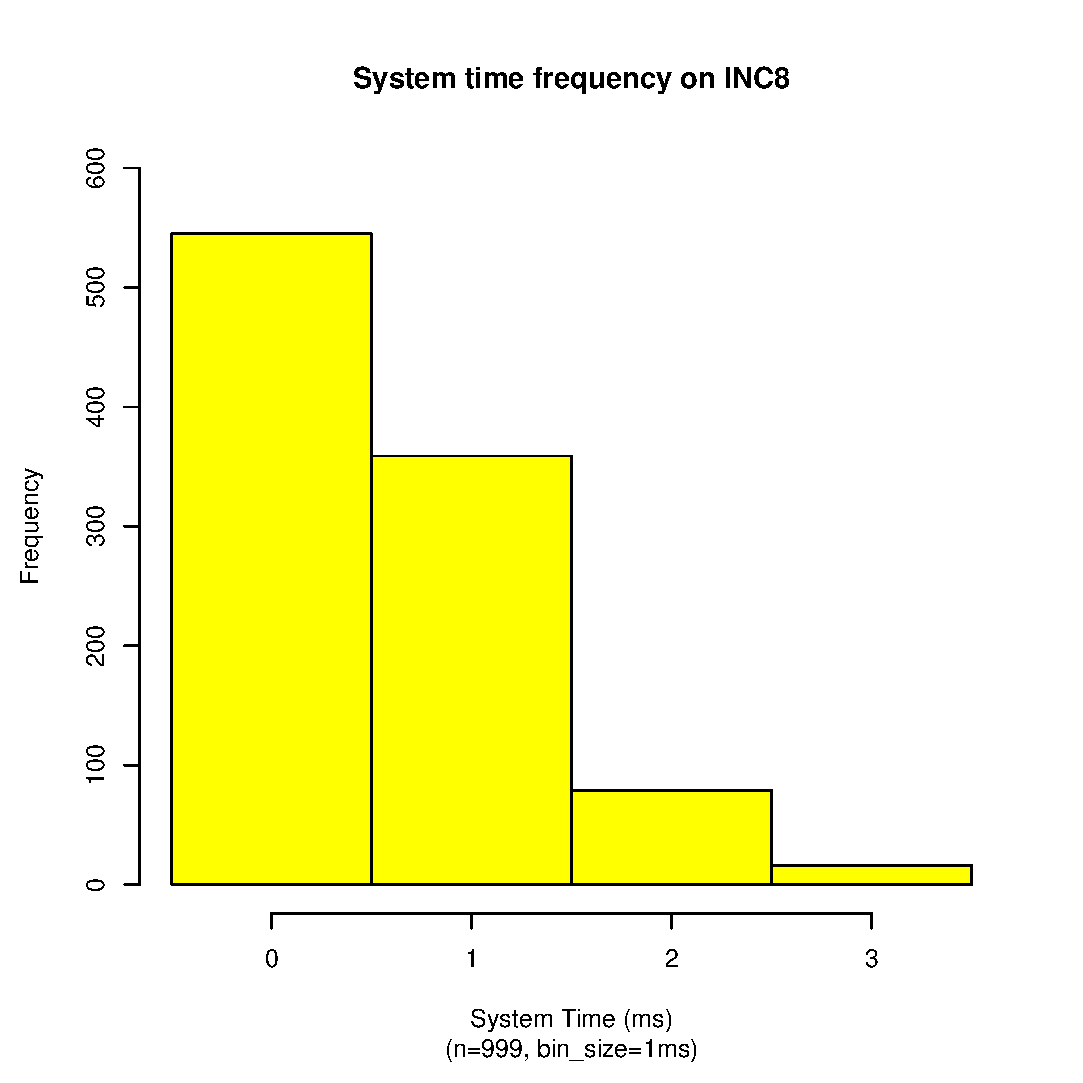
\includegraphics[scale=0.43]{u_s_time/8_sec_st_hist.eps}
		\label{fig:inc8_hist_st}
	}
	\caption{System Time Histograms of INC1 ... INC8~\label{fig:st_hist1}}
\end{figure}

\begin{figure}[hp!]
	\centering
	\subfigure[System time frequency on INC16]{
		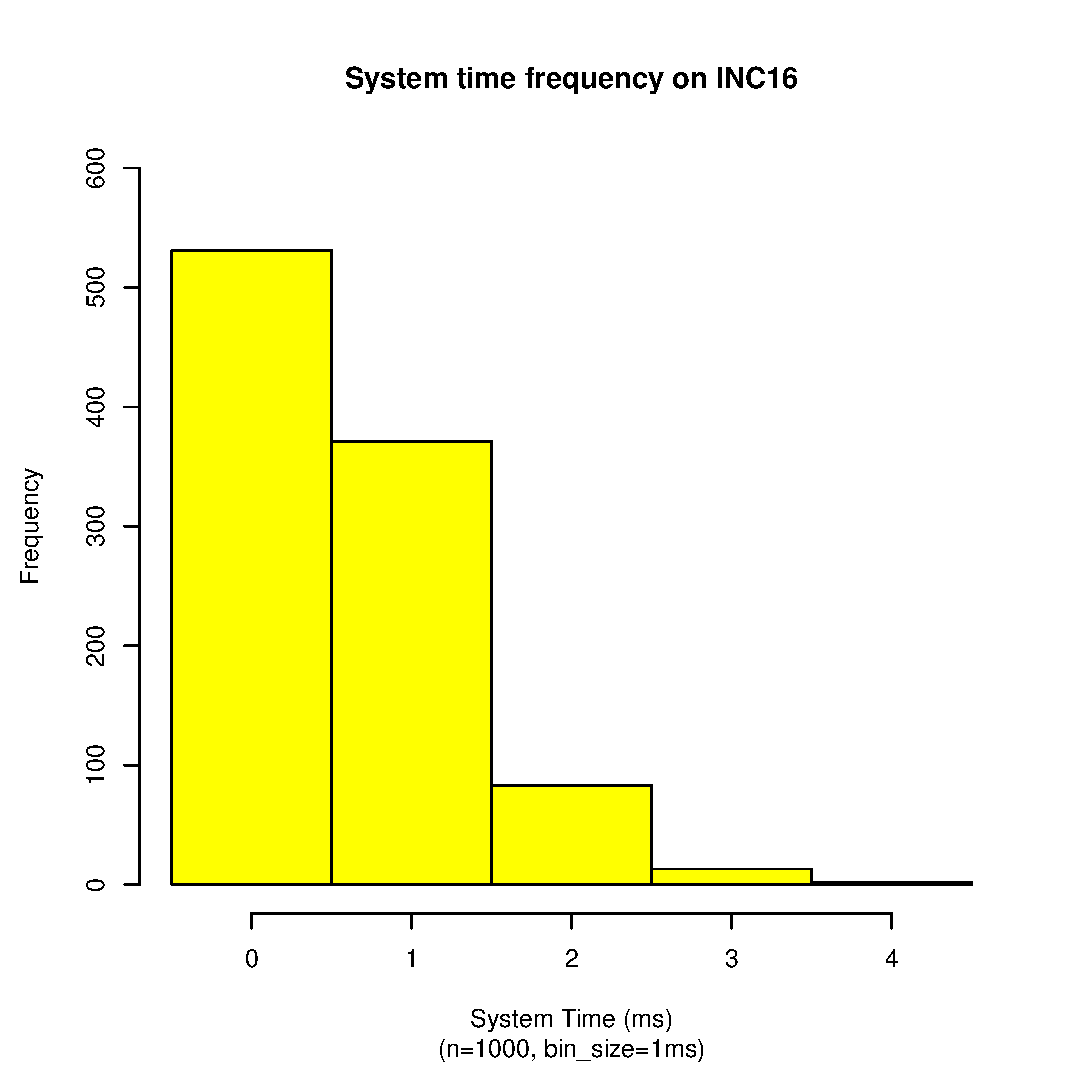
\includegraphics[scale=0.43]{u_s_time/16_sec_st_hist.eps}
		\label{fig:inc16_hist_st}
	}
	\subfigure[System time frequency on INC32]{
		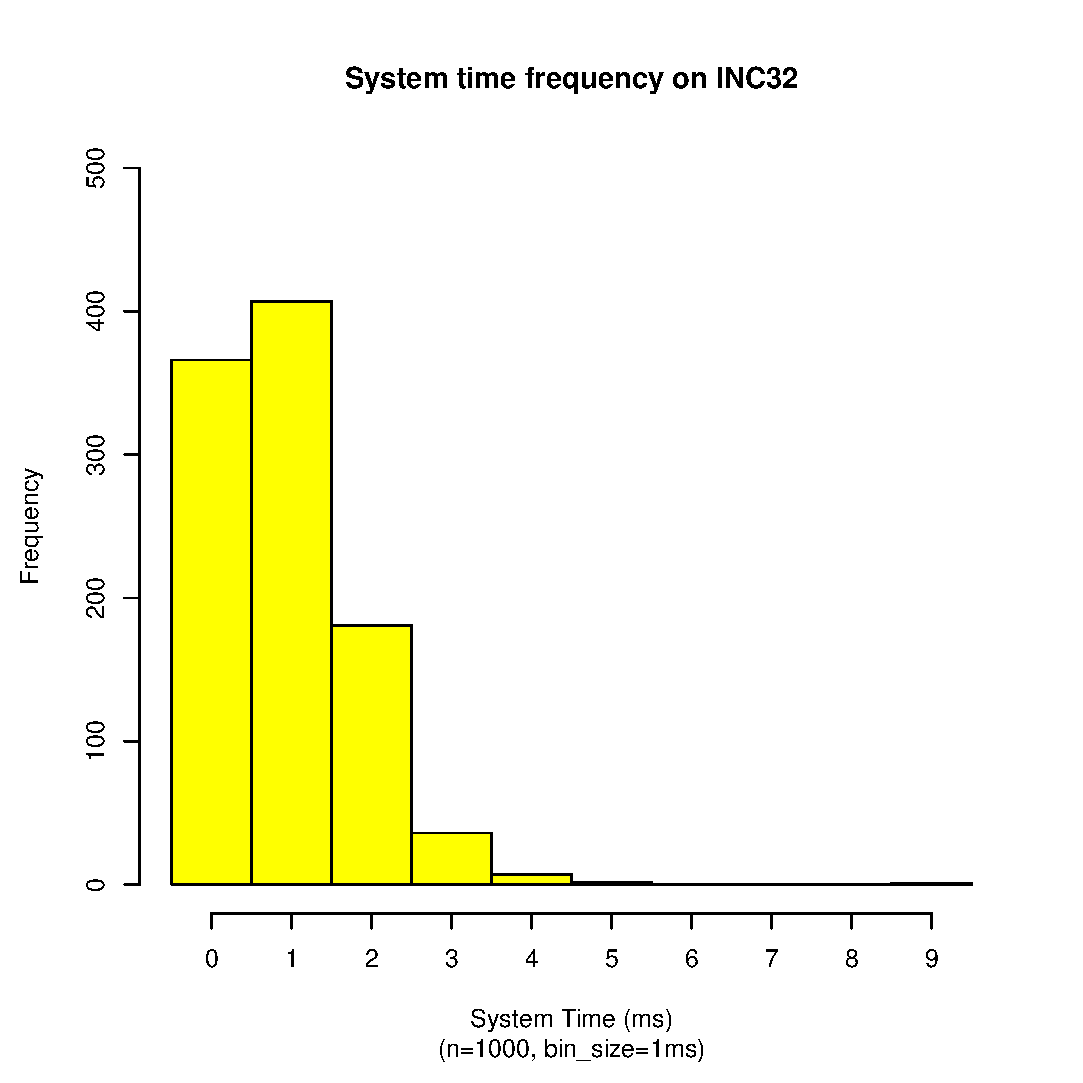
\includegraphics[scale=0.43]{u_s_time/32_sec_st_hist.eps}
		\label{fig:inc32_hist_st}
	}
	\subfigure[System time frequency on INC64]{
		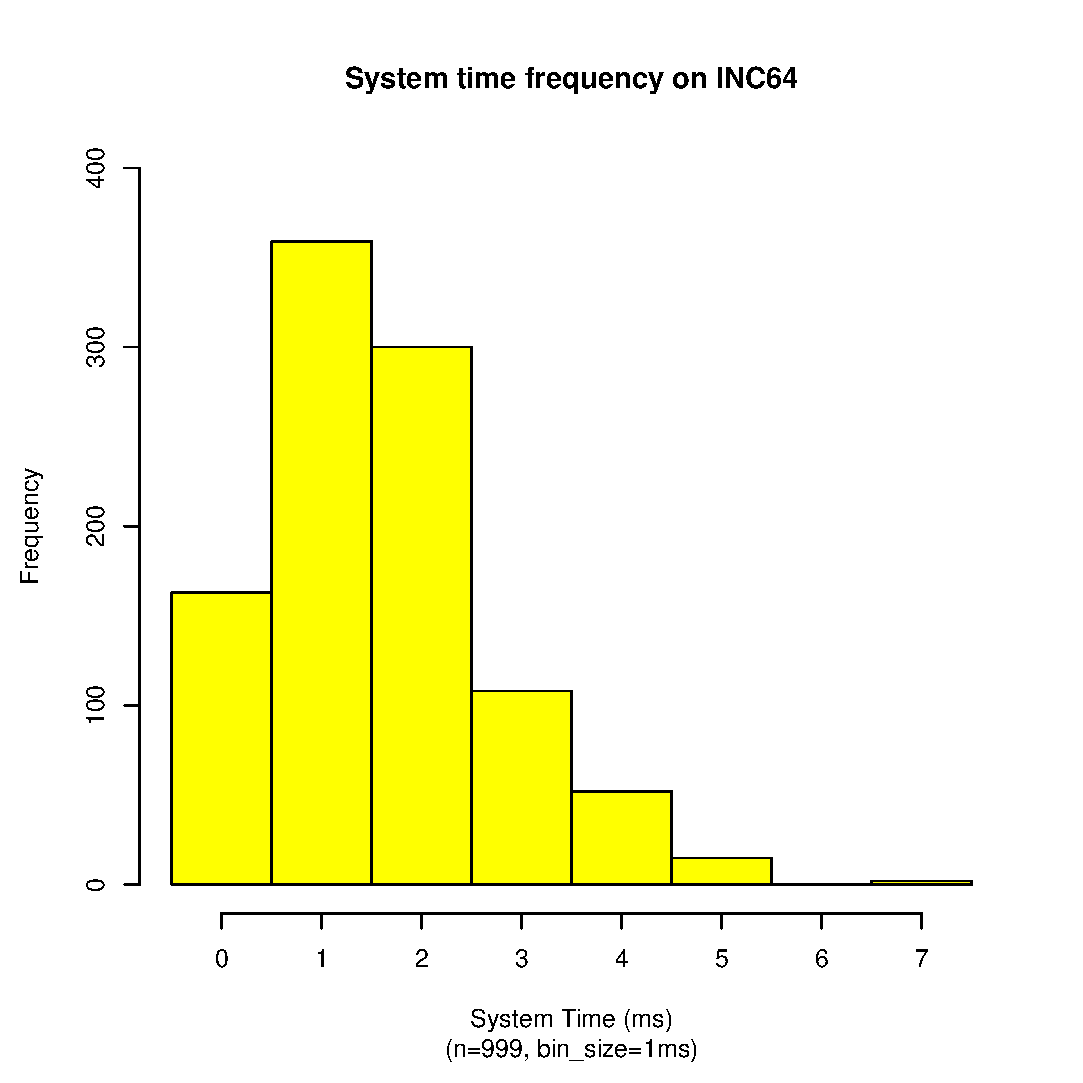
\includegraphics[scale=0.43]{u_s_time/64_sec_st_hist.eps}
		\label{fig:inc64_hist_st}
	}
	\caption{System Time Histograms of INC16 ... INC64\label{fig:st_hist2}}
\end{figure}

\begin{figure}[hp!]
	\centering
	\subfigure[System time frequency on INC128]{
		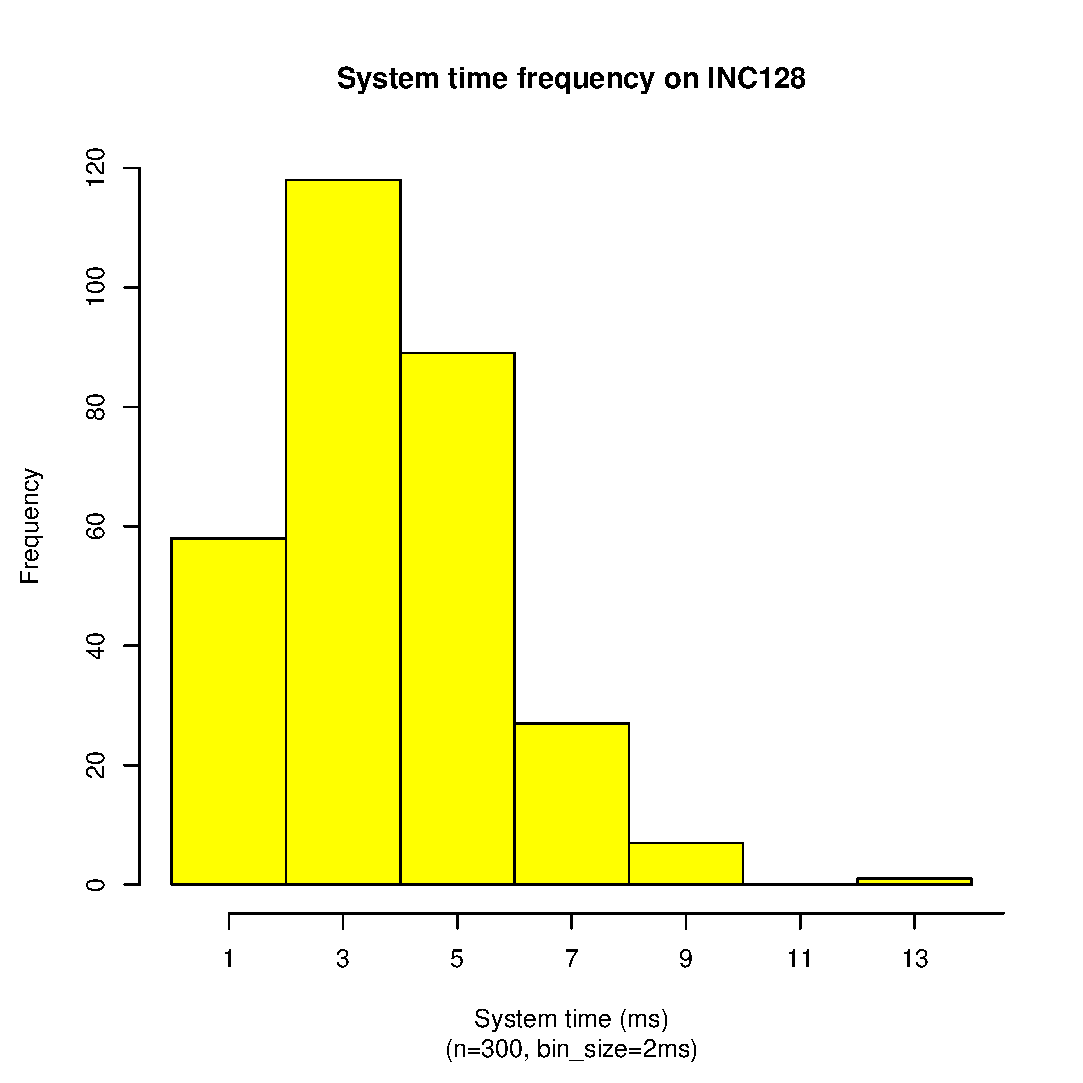
\includegraphics[scale=0.43]{u_s_time/128_sec_st_hist.eps}
		\label{fig:inc128_hist_st}
	}
	\subfigure[System time frequency on INC256]{
		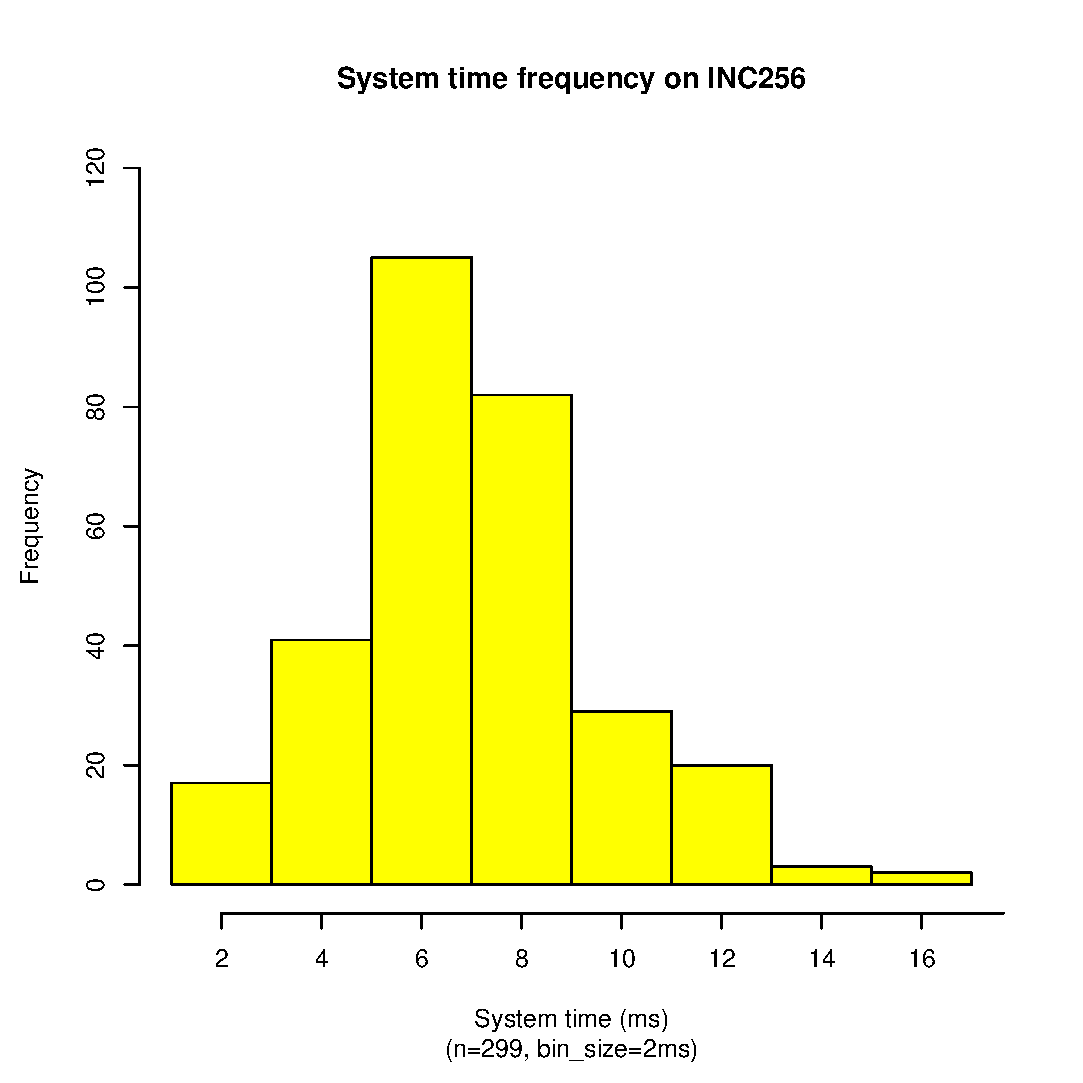
\includegraphics[scale=0.43]{u_s_time/256_sec_st_hist.eps}
		\label{fig:inc256_hist_st}
	}
	\subfigure[System time frequency on INC512]{
		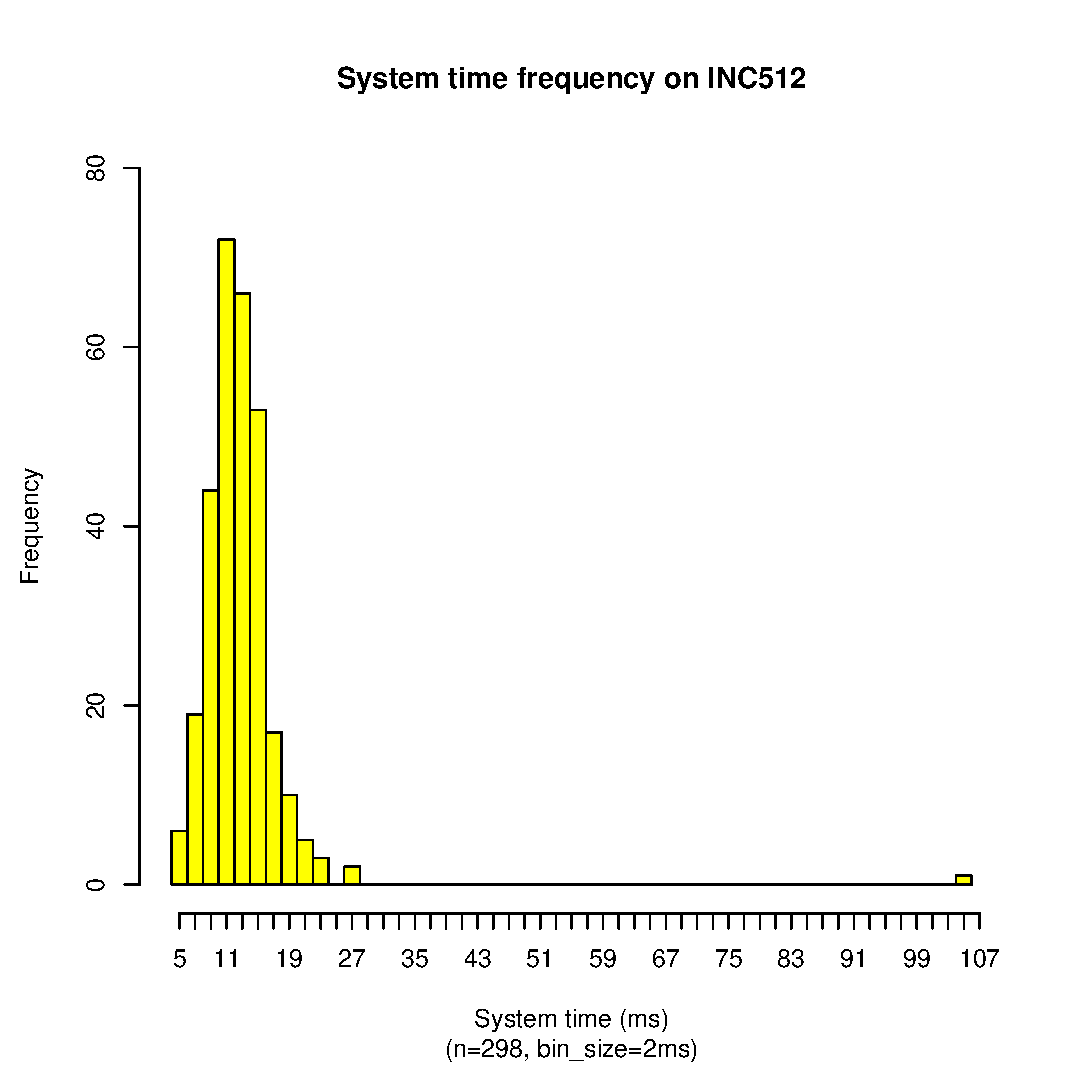
\includegraphics[scale=0.43]{u_s_time/512_sec_st_hist.eps}
		\label{fig:inc512_hist_st}
	}
	\subfigure[System time frequency on INC1024]{
		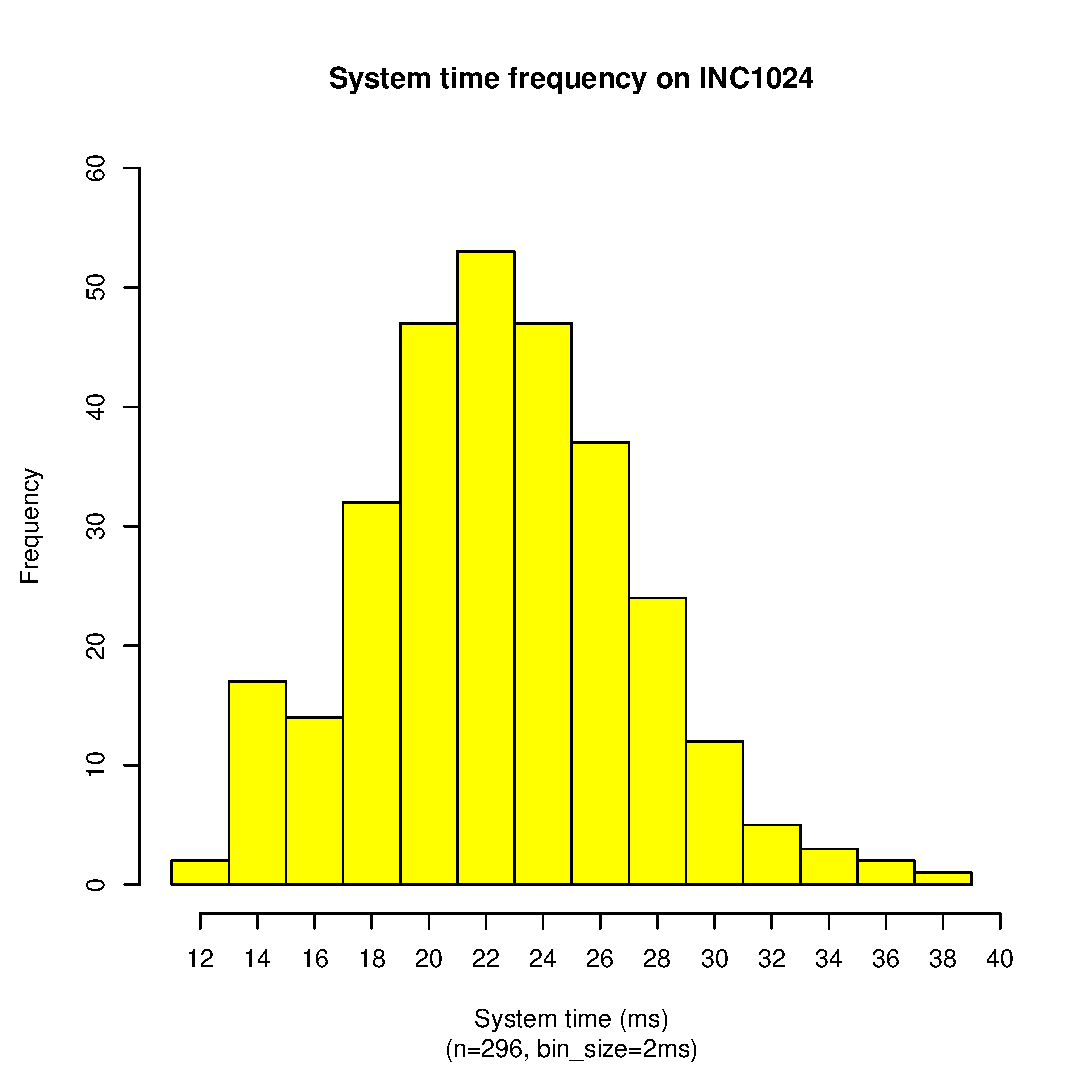
\includegraphics[scale=0.43]{u_s_time/1024_sec_st_hist.eps}
		\label{fig:inc1024_hist_st}
	}
	\caption{System Time Histograms of INC256 ... INC1024~\label{fig:st_hist3}}
\end{figure}

\begin{figure}[t]
	\centering
	\subfigure[System time frequency on INC2048]{
		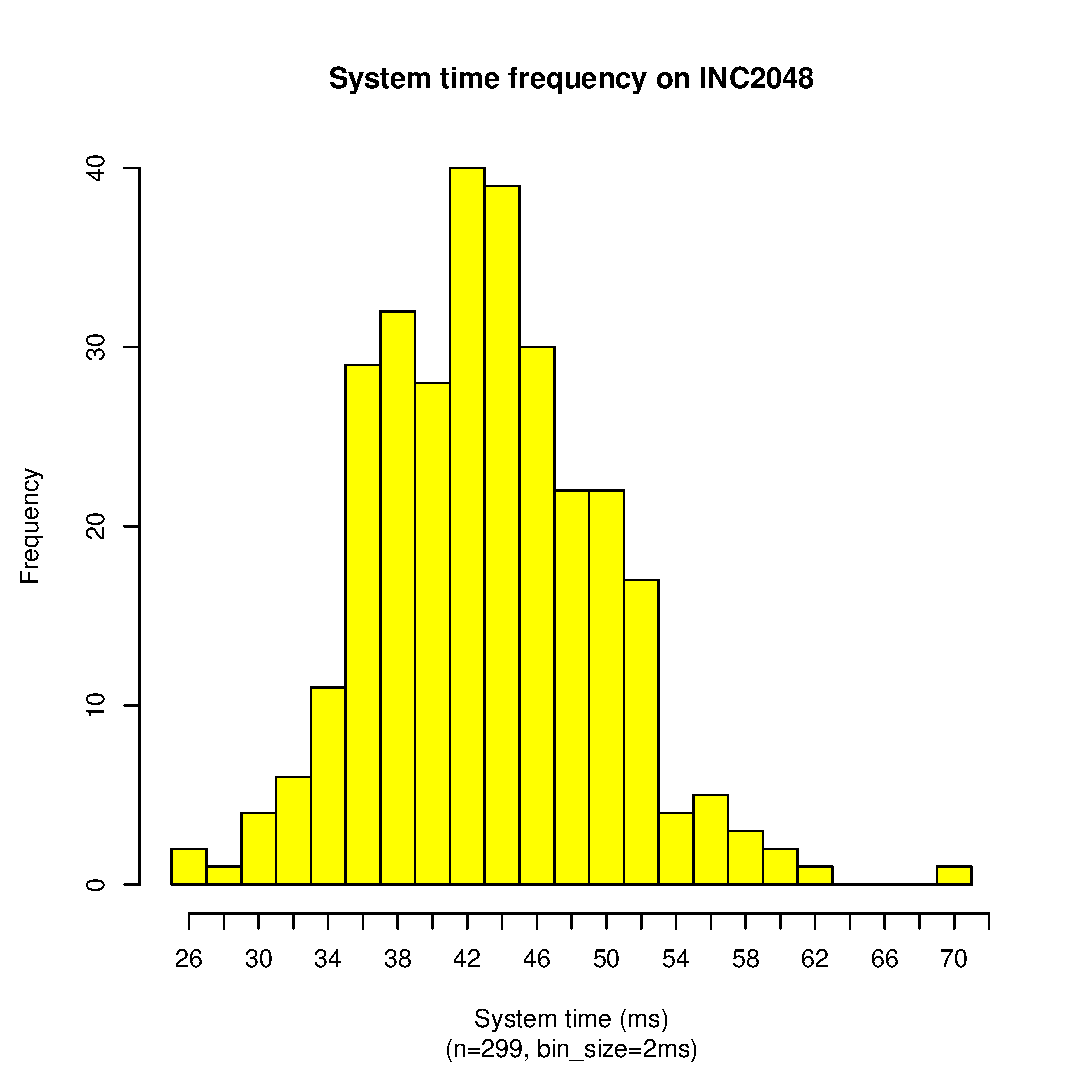
\includegraphics[scale=0.43]{u_s_time/2048_sec_st_hist.eps}
		\label{fig:inc2048_hist_st}
	}
	\subfigure[System time frequency on INC4096]{
		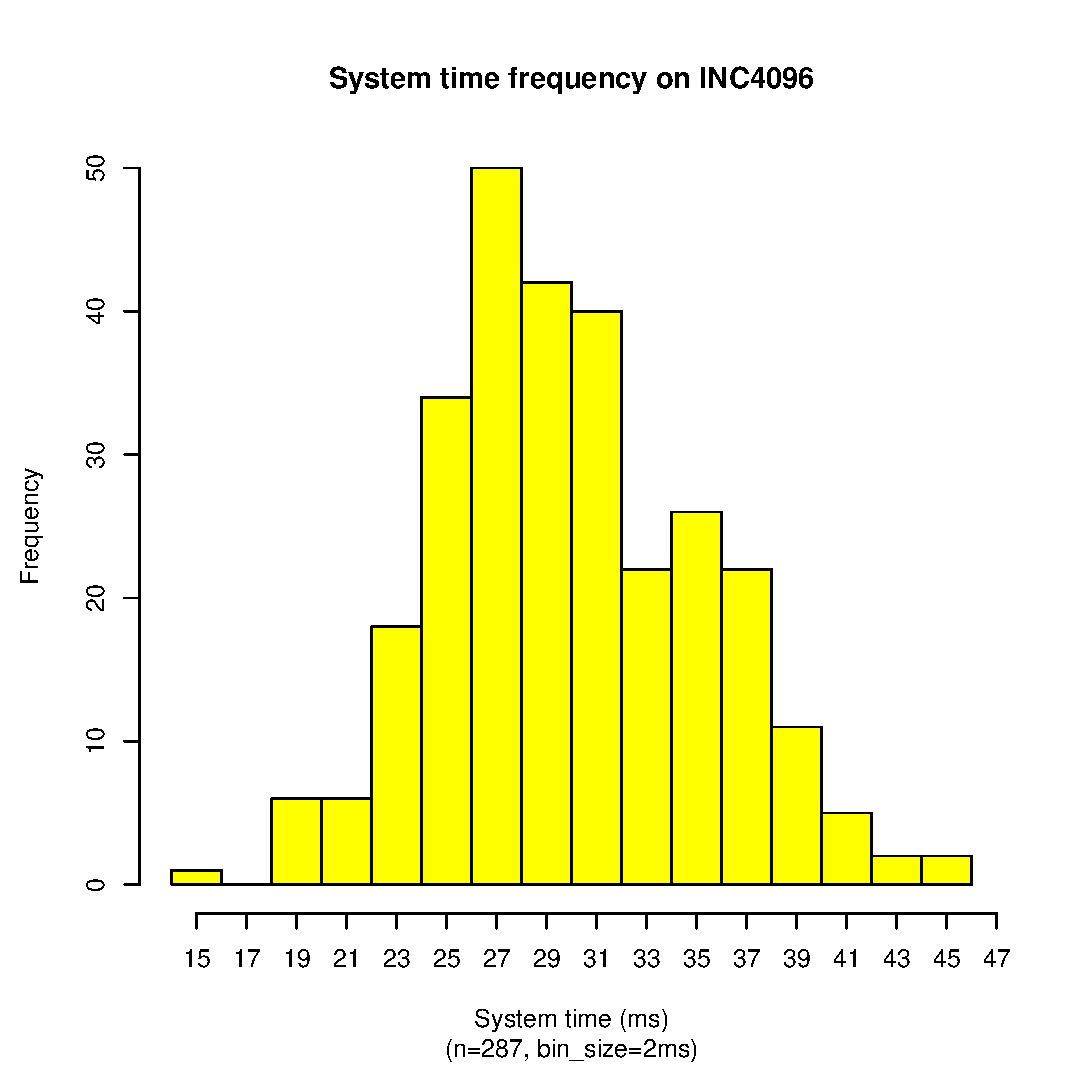
\includegraphics[scale=0.43]{u_s_time/4096_sec_st_hist.eps}
		\label{fig:inc4096_hist_st}
	}
	\caption{System Time Histograms of INC2048 and INC4096~\label{fig:st_hist4}}
\end{figure}

